%%%%%%%%%%%%%%%%%%%%%%%%%%%%%%%
%   Figures for chapter 5
%%%%%%%%%%%%%%%%%%%%%%%%%%%%%%%

\newcommand{\figProgressAgents}{
    \begin{figure}
        \centering
        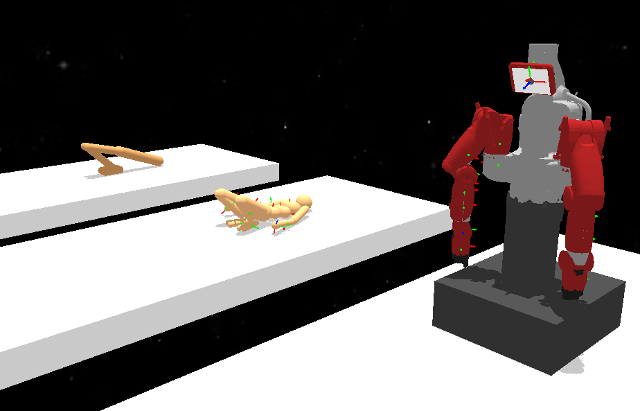
\includegraphics[width=0.9\textwidth]{./chapters/chapter_5/imgs/img_tysocmjc_agents.png}
        \caption{Current agent support. Currently the framework support mjcf
                 formats (from the mujoco engine)}
        \label{fig:ch5_progress_agents}
    \end{figure}
}

\newcommand{\figProgressSensors}{
    \begin{figure}
        \centering
        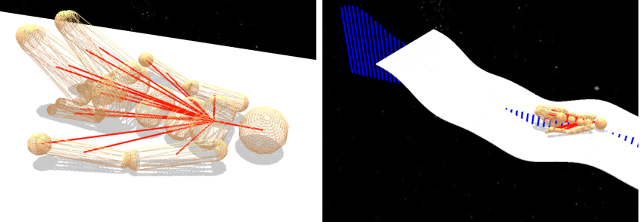
\includegraphics[width=0.9\textwidth]{./chapters/chapter_5/imgs/img_tysocmjc_sensors.png}
        \caption{Current sensor support. Currently the framework supports: 
                            a) intrinsic measurements (joint angles and velocities, body velocities and acceelrations, and relative positions).
                            b) extrinsic measurements (height fields taken from the terrain)}
        \label{fig:ch5_progress_sensors}
    \end{figure}
}

\newcommand{\figProgressTerrains}{
    \begin{figure}
        \centering
        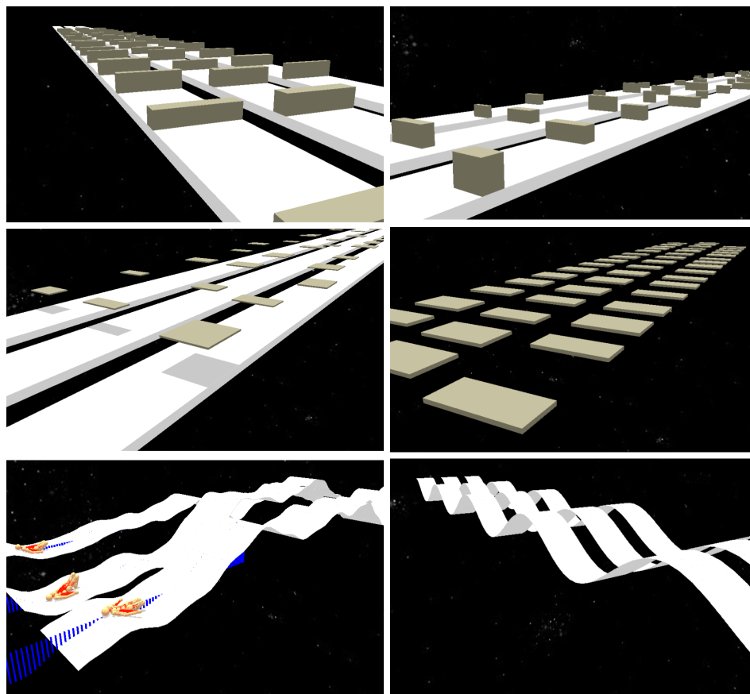
\includegraphics[width=0.9\textwidth]{./chapters/chapter_5/imgs/img_tysocmjc_terrains.png}
        \caption{Current terrain support. Currently the framework supports the
                 environments from \citeauthor{DeepmindEmergenceLocomotion}}
        \label{fig:ch5_progress_terrain}
    \end{figure}
}